\section{Background}\label{sec:background}
The NASA Viking missions in the 1970s were the first to successfully land on Mars, aiming to determine if life existed on the planet.
One experiment suggested the presence of life, but the results were ambiguous and inconclusive, and NASA was unable to repeat the experiment.
Nevertheless, these missions were deemed a monumental success and advanced our knowledge of the Martian environment~\cite{marsnasagov_vikings}.

Leveraging the knowledge gained from the Viking missions, NASA launched the \gls{mer} mission in 2003 to investigate whether Mars ever had the conditions to support life as we know it.
The mission landed two rovers, Spirit and Opportunity, on Mars in January 2004, and they quickly discovered clear evidence that water once flowed on Mars.
However, since water alone is not enough to support life, the next objective was to search for organic material as well~\cite{marsnasagov_observer, marsnasagov_spirit_opportunity}.

The Curiosity rover landed on Mars in August 2012 inside Gale Crater as part of the \gls{msl} mission with this very purpose.
Thanks to its sophisticated equipment, Curiosity was able to find evidence of past habitable environments on Mars based on chemical and mineral findings early in its mission~\cite{marsnasagov_msl}.

One of the instruments aboard the rover is the \gls{chemcam} instrument, which is a remote-sensing laser instrument used to gather \gls{libs} data from geological samples on Mars.
\gls{libs} is a technique that enables rapid analysis by using a laser to ablate and remove surface contaminants to expose the underlying material and generate a plasma plume from the now-exposed sample material~\cite{wiensChemcam2012}.
This plasma plume emits light that is captured through three distinct spectrometers to collect a series of spectral readings.
These spectra consist of emission lines that can be associated with the concentration of a specific element, and their intensity reflects the concentration of that element in the sample.
Consequently, a spectra serves as a complex, multi-dimensional fingerprint of the elemental composition of the examined geological samples~\cite{cleggRecalibrationMarsScience2017}.

\subsection{Baseline \& Replica}
For analyzing Martian geological samples, the \gls{chemcam} team currently uses the \gls{moc} model~\cite{cleggRecalibrationMarsScience2017}.
This model integrates \gls{pls} and \gls{ica} to predict the composition of major oxides.
The \gls{pls} and \gls{ica} phases of the \gls{moc} operate in parallel, and their predictions are blended to form the final predictions.
Though the \gls{moc} model has proven useful, it suffers from limitations in predictive accuracy and robustness.

An overview of the \gls{moc} model is shown in Figure~\ref{fig:moc_pipeline}.

\begin{figure}
	\centering
	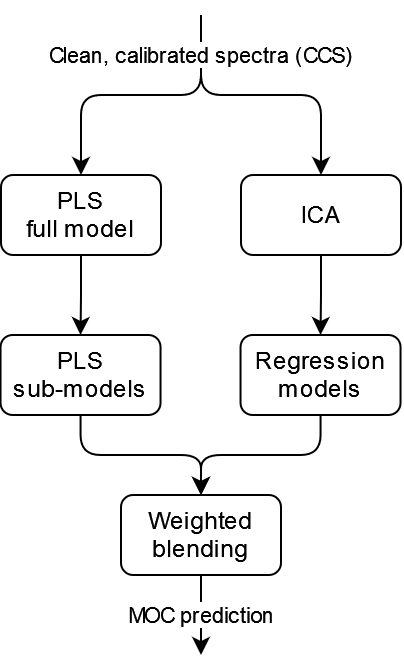
\includegraphics[width=0.225\textwidth]{images/moc_pipeline.png}
	\caption{Overview of the \gls{moc} model.}
	\label{fig:moc_pipeline}
\end{figure}

In \citet{p9_paper}, we presented our efforts to replicate the \gls{moc} model.
This effort was motivated by our desire to better understand the model and its performance, and to experiment with its components in order to determine how it could be improved.
However, as discussed in that paper, there were some differences between our replica and the original model.
These differences were caused by missing information in the original paper, and so rather than introducing our own assumptions, we designed experiments to determine the best way to replicate the model.

Initially, our replication omitted the use of the \gls{mad} for outlier removal in the data preprocessing stage, a step included in the original model.
To rectify this, we experimented with applying \gls{mad} at various stages in the pipeline.
We determined that its application post-removal of the initial five shots, and prior to masking and normalization, most closely mirrored the outcomes of the original model.

Furthermore, our replica only utilized a single dataset for the \gls{ica} phase, while the original model used all five datasets.
This difference was due to the original paper not specifying how the five datasets were used, and so we designed an experiment to determine how to use them in a way that would most closely replicate the original model.
We initially assumed that the datasets were aggregated and used as a single dataset.
This approach, however, did not align with the original model's results, likely due to the loss of information from the individual datasets.
Following this discovery, we instead used the datasets in the same way as we did in the \gls{pls1-sm} phase, which yielded results aligning more closely with the original model.

Finally, our initial replica used a random train/test split for training, in contrast to the original model's manual curation to ensure representation of extreme compositions in both sets.
This difference stemmed from the original authors' application of domain expertize in their dataset curation --- a process we could not directly replicate.
Nevertheless, we found that automatically identifying extreme compositions and ensuring that they were present in both the training and testing sets brought us closer to the original model.
We chose to pull out the $n$ largest and smallest samples by concentration range, for each oxide, and reserve them for the training set.
Then we would do a random split on the remaining dataset, such that the final train/test split would be a $80\%/20\%$ split.

With these changes, we created a more accurate replica of the \gls{moc} model, which we will use as our baseline for the rest of this paper.
As an additional measure, we have presented these changes to one of the original authors of~\citet{cleggRecalibrationMarsScience2017}, who confirmed that they were reasonable and in line with the original model's implementation.

Table~\ref{tab:replica_results_rmses} shows the \gls{rmse}s of the original models and our replicas after these changes.
Figure~\ref{fig:rmse_histograms} illustrates the distribution of these \gls{rmse}s as a grouped histogram.
The results show that the \gls{rmse}s of our replicas exhibit similar tendencies to the original models.
However, in some cases, our replicas have a lower \gls{rmse} than the original models, and in others, they have a higher \gls{rmse}.
These differences are due to a number of factors.

Firstly, the original models were trained with datasets from 1600mm and 3000mm standoff distances~\cite{cleggRecalibrationMarsScience2017}, while we only had access to the 1600mm dataset for our replicas.
Additionally, we automated the outlier removal for the PLS1-SM phase, unlike the original manual process.
As mentioned, the original authors manually curated their training and test sets, ensuring a broad elemental range, while we implemented an automatic process for our replicas due to lack of domain expertise.
Differences might also stem from varied implementation specifics, such as programming languages and libraries used.

\begin{table*}
	\centering
	\begin{tabular*}{\textwidth}{@{\extracolsep{\fill}}lllllll}
		\hline
		Element    & \gls{pls1-sm} (original) & PLS1-SM (replica) & \gls{ica} (original) & ICA (replica) & \gls{moc} (original) & \gls{moc} (replica) \\
		\hline
		\ce{SiO2}  & 4.33                     & 4.52              & 8.31                 & 8.66          & 5.30                 & 5.64                \\
		\ce{TiO2}  & 0.94                     & 0.50              & 1.44                 & 0.54          & 1.03                 & 0.48                \\
		\ce{Al2O3} & 2.85                     & 1.80              & 4.77                 & 3.37          & 3.47                 & 1.84                \\
		\ce{FeO_T} & 2.01                     & 1.94              & 5.17                 & 2.87          & 2.31                 & 1.82                \\
		\ce{MgO}   & 1.06                     & 0.91              & 4.08                 & 3.01          & 2.21                 & 1.56                \\
		\ce{CaO}   & 2.65                     & 1.77              & 3.07                 & 3.28          & 2.72                 & 2.09                \\
		\ce{Na2O}  & 0.62                     & 0.82              & 2.29                 & 2.11          & 0.62                 & 1.34                \\
		\ce{K2O}   & 0.72                     & 0.73              & 0.98                 & 1.37          & 0.82                 & 1.16                \\
		\hline
	\end{tabular*}
	\caption{\gls{rmse}s of the original and our replicas of the \gls{pls1-sm}, \gls{ica}, and \gls{moc} models.}
	\label{tab:replica_results_rmses}
\end{table*}

\begin{figure*}
	\centering
	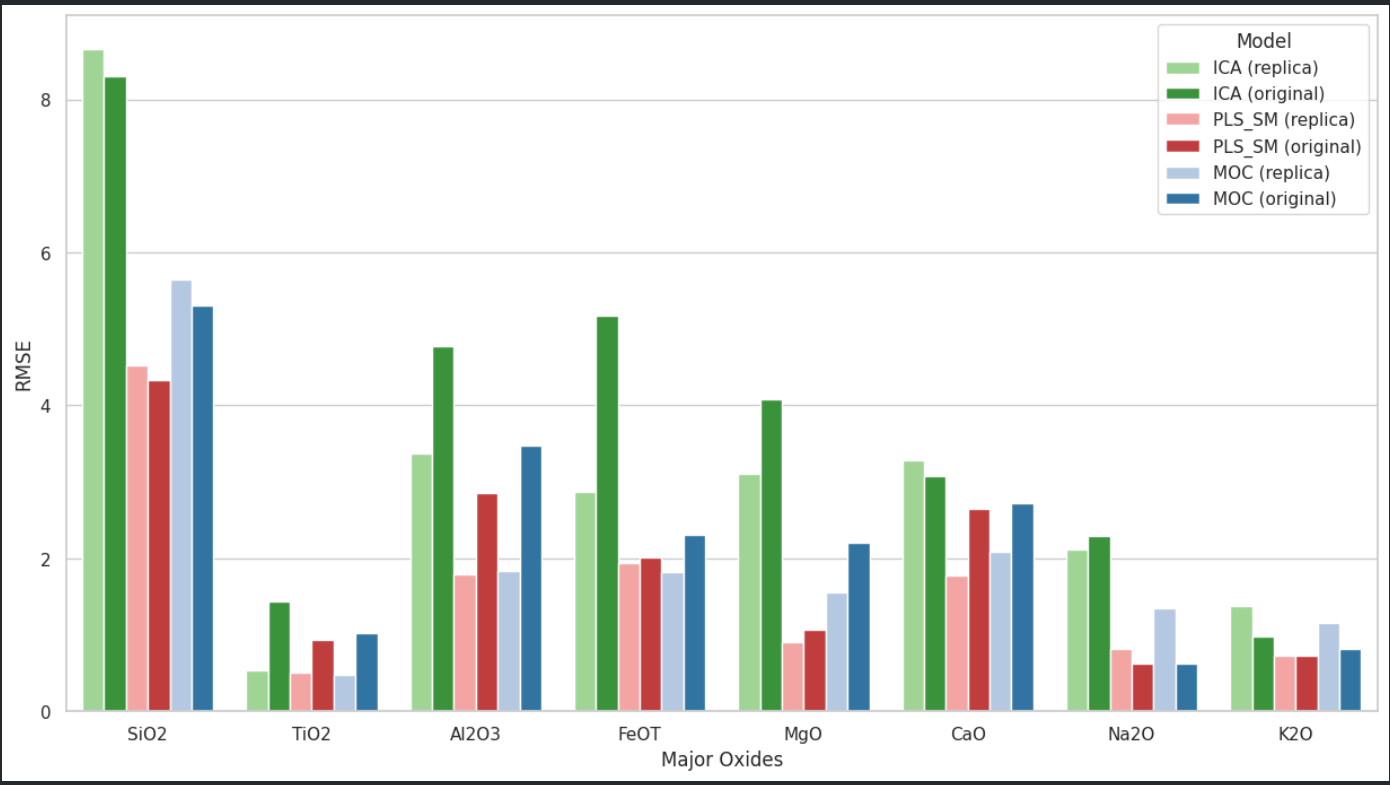
\includegraphics[width=0.85\textwidth]{images/rmse_historgram.png}
	\caption{Grouped histogram of the \gls{rmse}s of the original and our replicas of the \gls{pls1-sm}, \gls{ica}, and \gls{moc} models.}
	\label{fig:rmse_histograms}
\end{figure*}

Through a series of comparative experiments, we showed that the model selection was the primary cause of these limitations, and we showed how both \gls{ann} and \gls{gbr} methods could be used to improve the model's predictive accuracy and robustness.
This is further underscored by work from the SuperCam team.
In 2021, the Perseverance rover landed on Mars, equipped with the SuperCam instrument, which is the successor to the \gls{chemcam} instrument.
As part of the ongoing work to support the SuperCam instrument, \citet{andersonPostlandingMajorElement2022} experimented with various machine learning models to predict the composition of major oxides in geological samples using the SuperCam \gls{libs} calibration dataset.
While the team decided to retain \gls{pls} for analyzing certain oxides, \gls{ica} was entirely discontinued.
Instead, models based on \gls{gbr}, \gls{rf}, and \gls{lasso} were selected for other oxides.
This decision reinforces our finding that \gls{ica} regression models fall short in accurately predicting the composition of major oxides in geological samples.
Consistent with our observations, \gls{gbr} was also identified as a high-performing model in their analyses.